% ****** Start of file apssamp.tex ******
%
%   This file is part of the APS files in the REVTeX 4.1 distribution.
%   Version 4.1r of REVTeX, August 2010
%
%   Copyright (c) 2009, 2010 The American Physical Society.
%
%   See the REVTeX 4 README file for restrictions and more information.
%
% TeX'ing this file requires that you have AMS-LaTeX 2.0 installed
% as well as the rest of the prerequisites for REVTeX 4.1
%
% See the REVTeX 4 README file
% It also requires running BibTeX. The commands are as follows:
%
%  1)  latex apssamp.tex
%  2)  bibtex apssamp
%  3)  latex apssamp.tex
%  4)  latex apssamp.tex
%
\documentclass[%
 reprint,
%superscriptaddress,
%groupedaddress,
%unsortedaddress,
%runinaddress,
%frontmatterverbose, 
%preprint,
%showpacs,preprintnumbers,
%nofootinbib,
%nobibnotes,
%bibnotes,
 amsmath,amssymb,
 aps,
%pra,
%prb,
%rmp,
%prstab,
%prstper,
%floatfix,
]{revtex4-1}

\usepackage{graphicx}% Include figure files
\usepackage{dcolumn}% Align table columns on decimal point
\usepackage{bm}% bold math
%\usepackage{hyperref}% add hypertext capabilities
%\usepackage[mathlines]{lineno}% Enable numbering of text and display math
%\linenumbers\relax % Commence numbering lines

%\usepackage[showframe,%Uncomment any one of the following lines to test 
%%scale=0.7, marginratio={1:1, 2:3}, ignoreall,% default settings
%%text={7in,10in},centering,
%%margin=1.5in,
%%total={6.5in,8.75in}, top=1.2in, left=0.9in, includefoot,
%%height=10in,a5paper,hmargin={3cm,0.8in},
%]{geometry}

\begin{document}

\preprint{APS/123-QED}

\title{A New Novel Trap For Neutral Atoms}% Force line breaks with \\
\thanks{A footnote to the article title}%

\author{D. Lobser}
 \altaffiliation[Also at ]{Physics Department, XYZ University.}%Lines break automatically or can be forced with \\
%\author{Second Author}%
 %\email{Second.Author@institution.edu}
%\affiliation{%
 %Authors' institution and/or address\\
 %This line break forced with \textbackslash\textbackslash
%}%

%\collaboration{MUSO Collaboration}%\noaffiliation

%\author{Charlie Author}
 %\homepage{http://www.Second.institution.edu/~Charlie.Author}
%\affiliation{
 %Second institution and/or address\\
 %This line break forced% with \\
%}%
%\affiliation{
 %Third institution, the second for Charlie Author
%}%
%\author{Delta Author}
%\affiliation{%
 %Authors' institution and/or address\\
 %This line break forced with \textbackslash\textbackslash
%}%
%
%\collaboration{CLEO Collaboration}%\noaffiliation

\date{\today}% It is always \today, today,
             %  but any date may be explicitly specified

\begin{abstract}
A modification to the standard Time-averaged Orbiting Potential (TOP) trap that allows for very isotropic potentials.
\begin{description}
\item[Usage]
Secondary publications and information retrieval purposes.
\item[PACS numbers]
May be entered using the \verb+\pacs{#1}+ command.
\item[Structure]
You may use the \texttt{description} environment to structure your abstract;
use the optional argument of the \verb+\item+ command to give the category of each item. 
\end{description}
\end{abstract}

\pacs{Valid PACS appear here}% PACS, the Physics and Astronomy
                             % Classification Scheme.
%\keywords{Suggested keywords}%Use showkeys class option if keyword
                              %display desired
\maketitle

%\tableofcontents

\section{\label{sec:level1} Introduction}
%The Time-averaged Orbiting Potential (TOP) trap was developed in 1993 for the creation of the first Bose-Einstein condensate (BEC). Since the first realization of BEC, numerous magnetic traps have been developed which displace the magnetic zero away from the trap center. The TOP trap is able to generate the extremely cylindrical potentials necessary for vortex experiments where the roundness of the trap was critical for maintaining the large angular momentum of the condensate. In the strong field limit, the axial and radial spring constants have a ratio of $\sqrt{8}$. By reducing the strength of the quadrupole field, gravitational effects cause this ratio to decrease, allowing for a spherical potential. However, construction asymmetries can only be shimmed out in the xy plane preventing full control over the ellipsoidal shape of the potential. Through the addition of a third oscillating field, we gain control over all of the elliptic cross terms allowing for an extremely isotropic potential.

Over a century ago, Boltzmann derived his famous H-theorem to describe entropy using mechanical arguments. His theories met with a vicious opposition because the time reversal symmetry inherent to mechanical systems conflicted with the irreversible nature of entropy. This was said to have aggravated his bouts of depression and ultimately led to his suicide in 1906. In a series of heated articles, Boltzmann did acknowledge that certain exotic cases exist that could lead to bizarre collective behavior but dismissed them as irrelevant to the description of naturally occurring systems. One case in particular was that a gas confined to a perfectly spherical harmonic potential wouldn't necessarily reach equilibrium. Namely, the monopole motion of the gas is \textit{undamped}. Experimental study of this particular phenomenon has so far been prevented by the difficulty in generating a sufficiently isotropic harmonic potential. 



%This opposition to Boltzmann's views was said to have aggravated his bouts of depression and ultimately led to his suicide in 1906. 

%Over a century ago, Boltzmann developed his transport equation to describe how gaseous systems reach equilibrium, which ultimately led to a model of the 2nd law of thermodynamics known as the H-theorem. His theories met with a vicious opposition because they derived from mechanical arguments and the inherent time reversal symmetry of mechanical systems conflicted with the irreversible nature of entropy. This opposition to Boltzmann's views was said to have aggravated his bouts of depression and in 1906 he committed suicide. Boltzmann never wavered in his views and adamantly defended the validity of his approach. Despite the arguments against his theories, he explicitly showed that a gas confined in a spherical harmonic potential won't necessarily reach equilibrium. In particular, the monopole, or ``breathe'' mode, of a gas is expected to be completely \textit{undamped}. This effect has never been experimentally verified because of the difficulty in creating a spherical harmonic potential. We have developed a new magnetic trap which is capable of generating a potential which is spherical to within 99.9\%

The theoretical issues which fueled the debate stem from the Boltzmann equation. For a phase space distribution,  $f \equiv f\left(\mathbf{r},\mathbf{p},t\right)$, the Boltzmann equation in its simplest form is
\begin{equation}
\frac{df}{dt} = I_{coll}\left[f\right],
\end{equation}
where $I_{coll}\left[f\right]$ is a collision function, referred to as the \textit{collision integral}. Essentially, the Boltzmann states that the phase space distribution of a gas approaches equilibrium at a rate proportional to the frequency of collisions. At equilibrium, the distribution becomes stationary and the collision integral vanishes. Expanding the derivative and including the explicit definition of  $I_{coll}\left[f\right]$ leads to the more standard form of the Boltzmann equation

%where $f \equiv f\left(\mathbf{r},\mathbf{p},t\right)$ is the probability density of finding a particle at a given phase space coordinate, and $I_{coll}\left[f\right]$ is a collision function. Essentially, the Boltzmann equation states that the distribution of particles in a gas approaches equilibrium at a rate proportional to the frequency of collisions. When equilibrium is reached, the distribution becomes stationary and the collisional contribution vanishes. Expanding the derivative and including the explicit definition of $I_{coll}\left[f\right]$, the Boltzmann equation takes on the more standard form

%In a confining potential, the distribution takes on a spatial dependence and $f = f\left(\mathbf{r},\mathbf{p},t\right)$. Expanding the derivative and including the explicit definition of $I_{coll}\left[f\right]$, the Boltzmann equation takes on the more standard form
%\begin{eqnarray}
%\frac{\partial f}{\partial t} + \mathbf{v}_1\cdot\nabla_\mathbf{r}f+\frac{\mathbf{F}}{m}\cdot\nabla_{\mathbf{v}_1}f = \frac{\sigma_0}{4\pi} \int d^2\Omega d^3\mathbf{v}_2\left|\mathbf{v}_2-\mathbf{v}_1\right|\left(f_1'f_2'-f_1f_2\right)~~~~~~~~~~~~~~~~~ \nonumber\\
% \times \delta\left(\mathbf{p}_1+\mathbf{p}_2 - \mathbf{p}_1'-\mathbf{p}_2'\right)   \delta\left(p_1^2+p_2^2 - p_1'^2-p_2'^2\right)
%\end{eqnarray}
%Typically, energy and momentum conservation is implicitly assumed and the delta functions are omitted in the standard literature.
\begin{eqnarray}
\frac{\partial f}{\partial t}&+&\mathbf{v}_1\cdot\nabla_\mathbf{r}f+\frac{\mathbf{F}}{m}\cdot\nabla_{\mathbf{v}_1}f = \label{eq:boltzmann}\\
& &\frac{\sigma_0}{4\pi} \int d^2\Omega d^3\mathbf{v}_2\left|\mathbf{v}_2-\mathbf{v}_1\right|\left(f(\mathbf{v}_1')f(\mathbf{v}_2')-f(\mathbf{v}_1)f(\mathbf{v}_2)\right)\nonumber
\end{eqnarray}
where $\sigma_0$ is the collision cross section. Energy and momentum conservation are implicitly assumed, but could easily be included in the collision integral using a delta function. The other major assumption is that the atoms can be treated as hard spheres, but this approximation is valid for \textit{s}-wave collisions when mean field effects are negligible and the cloud is non-degenerate. %As the cloud becomes highly degenerate, Bose enhancement terms must be taken into account and Eq.~\ref{eq:boltzmann} becomes
%\begin{equation}
%\frac{\partial f}{\partial t} + \mathbf{v}_1\cdot\nabla_\mathbf{r}f+\frac{\mathbf{F}}{m}\cdot\nabla_{\mathbf{v}_1}f =\frac{\sigma_0}{4\pi}\int d^2\Omega d^3\mathbf{v}_2\left|\mathbf{v}_2-\mathbf{v}_1\right|\left(f_1'f_2'(1+h^3f_1)(1+h^3f_2)-f_1f_2(1+h^3f_1')(1+h^3f_2')\right).
%\label{eq:boltzmann}
%\end{equation}
%The distribution functions in the Bose enhancement terms are scaled by $h^3$ where $h$ is Planck's constant, and for a thermal cloud the enhancement terms are approximately unity.

Distributions of the form
\begin{equation}
\log f = \alpha + \mathbf{\beta}\cdot\mathbf{v}+\gamma v^2
\label{eq:collisioninvariant}
\end{equation}
cause the collision integral to vanish due to conservation of energy and momentum and are referred to as \textit{collisionally invariant}. These distributions, generally called \textit{local equilibrium distributions}, do not necessarily satisfy Eq.~\ref{eq:boltzmann} and constraints must be placed on $\alpha$, $\beta$, and $\gamma$. For a sufficiently general outside potential, these constants can be constrained to produce an equilibrium distribution equivalent to Maxwell-Boltzmann. For certain special potentials, collisionally invariant distributions exist that satisfy Eq.~\ref{eq:boltzmann}. For an isotropic harmonic potential, the solution is essentially an equilibrium distribution undergoing temperature oscillations where the spatial distribution varies identically such that the distribution satisfies the equilibrium constraint at each point in time. Persistence of monopole oscillations can be described in various ways, but can be elucidated by the two particle case. 

In the presence of spherical symmetry, the problem can be treated as analogously one dimensional and the radial motion of a single particle of mass $m$, energy $E$ and angular momentum $L$ is governed by the effective potential
\begin{equation}
V_e = \frac{L^2}{2mr^2}+\frac{1}{2}m\omega^2r^2.
\end{equation}
The radial force,
\begin{equation}
m\frac{d^2r}{dt^2} = -\frac{d}{dr}V_e,
\label{eq:radialforce}
\end{equation}
can be combined with the kinetic energy,
\begin{equation}
\frac{1}{2}m\left(\frac{dr}{dt}\right)^2 = E-V_e,
\end{equation}
by integrating Eq.~\ref{eq:radialforce}. This yields
\begin{equation}
\frac{d^2}{dt^2}r^2 = -\Omega^2\left(r^2-r_0^2\right),
\end{equation}
where $\Omega\equiv2\omega$ and $r_0^2=E/(m\omega^2)$, so that the square radius undergoes sinusoidal oscillations around its mean value $r_0^2$ at a frequency of $2\omega$. If there are 2 particles, 1 and 2, each with individual values of E, L and $r^2$, each particle will oscillate at $2\omega$ and taking the linear combination of their respective differential equations yields
\begin{equation}
\frac{d^2}{dt^2}r_t^2 = -\Omega^2\left(r_t^2-r_{0t}^2\right)
\label{eq:monopolecomb}
\end{equation}
so their combined square radius, $r_t^2 = r_1^2+r_2^2$, oscillates around its mean value, $r_{0t}^2 = (E_1+E_2)/(m\omega^2)$. The magnitude of the monopole motion depends on the magnitude and relative phase of the individual particle trajectories. These individual quantities will abruptly change in the event of a collision. Assuming the collisions are local, $r_1$, $r_2$ and thus $r_t^2$ will not change from the instant before to the instant after the collision. Similarly, momentum and energy conservation imply that $\frac{d}{dt}r_t^2$ and $r_{0t}^2$ are unchanged by the collision. These three continuities imply that the parameters and boundary conditions of Eq.~\ref{eq:monopolecomb} are matched directly before and after a collision. This ensures that neither the magnitude or phase of the oscillation will change as the result of a pairwise collsion. Generalizing to N atoms, so that
\begin{equation}
r_t^2 = \sum_{i=1}^Nr_i^2
\end{equation}
and
\begin{equation}
r_{0t}^2 = \frac{1}{m\omega^2}\sum_{i=1}^NE_i,
\end{equation}
one can see that the monopole mode is left unperturbed -- and in particular \textit{undamped} -- by local, pairwise, momentum- and energy-conserving collisions.







The system becomes integrable and the energy in the monopole mode is a conserved quantity.



  

\begin{figure}[htb]

    \begin{center}
    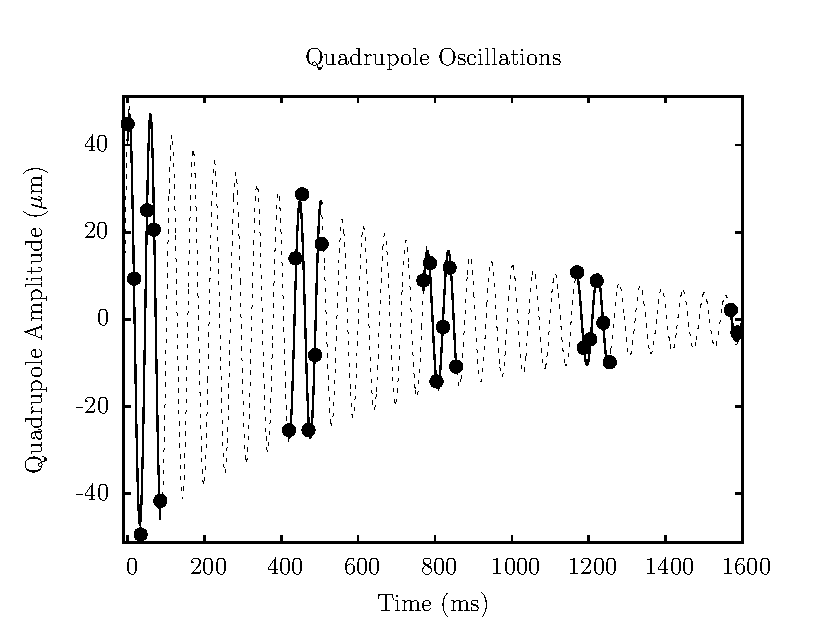
\includegraphics[width=40mm]{./figs/725QuadDecay.pdf}
    %${}^{}$ 
    %${}^{}$ 
    %${}^{}$
    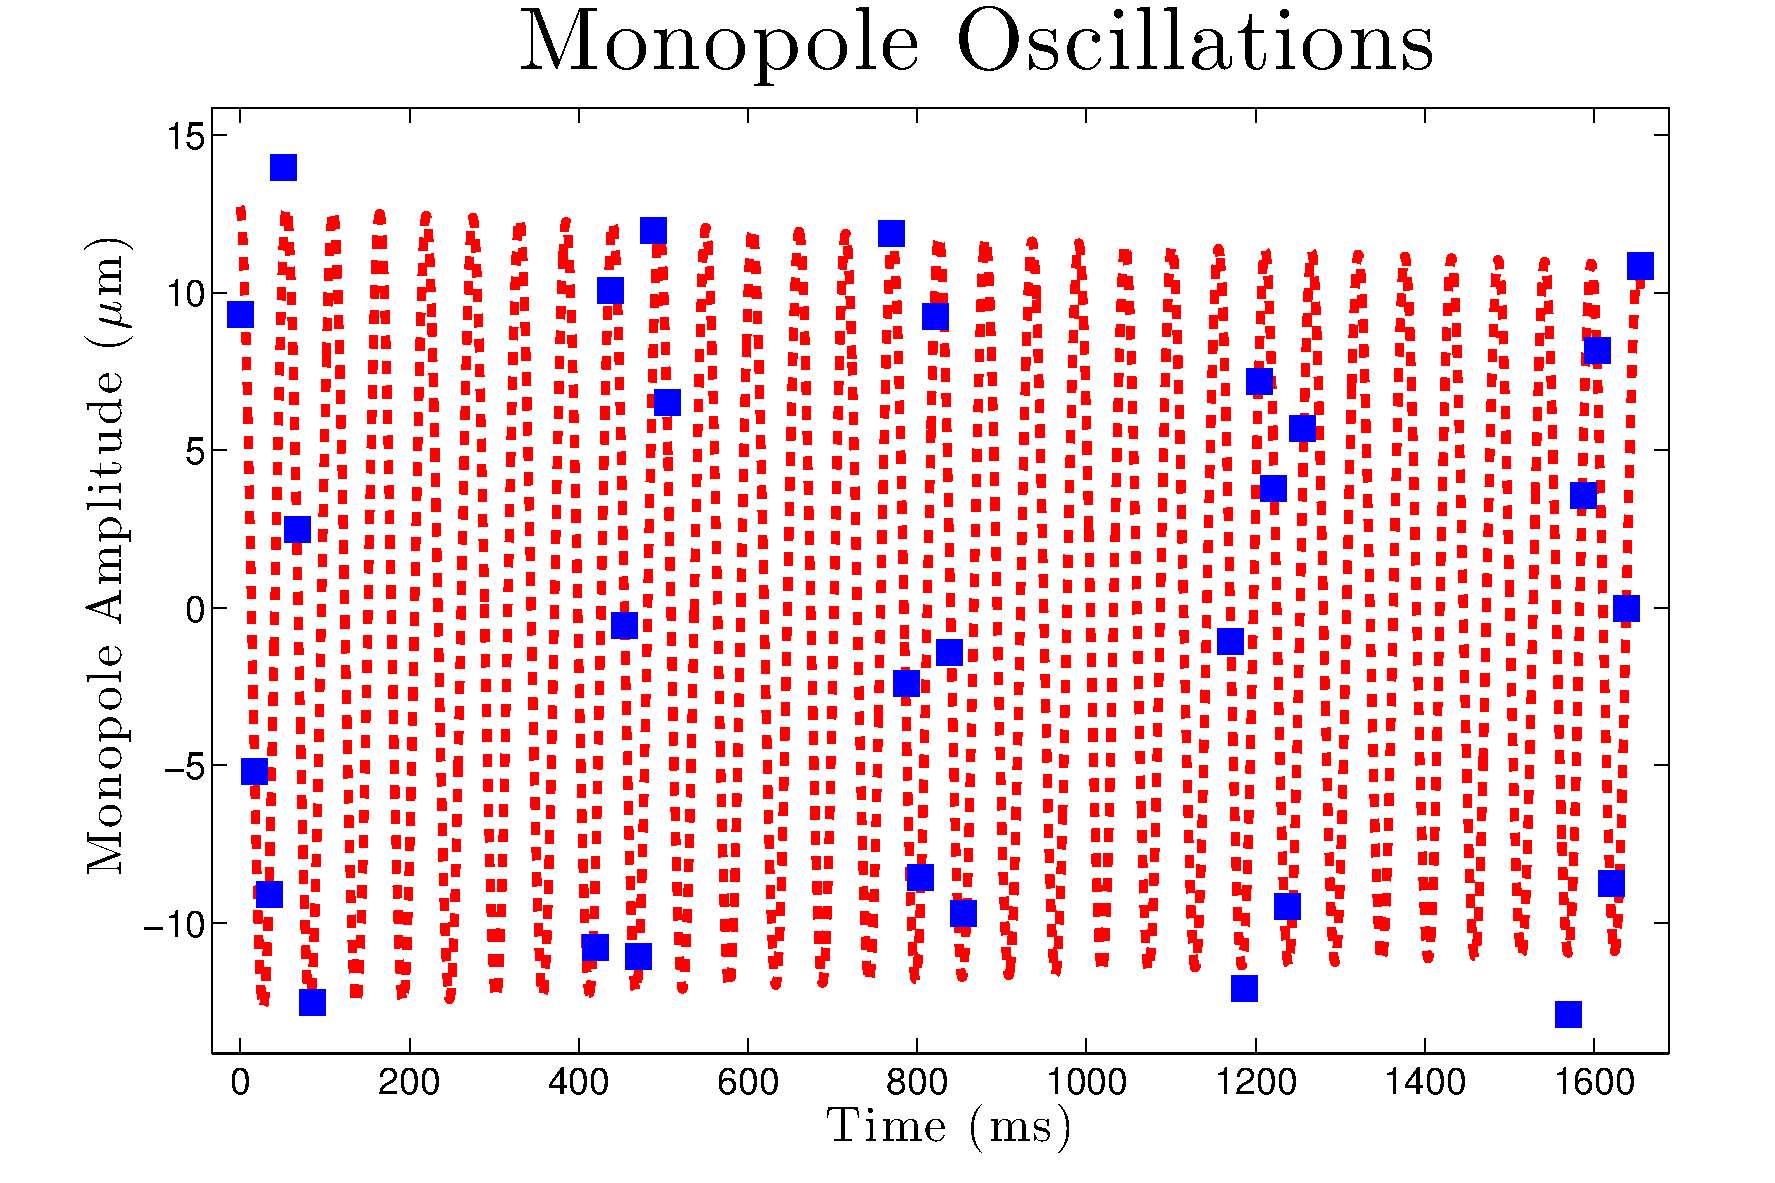
\includegraphics[width=40mm]{./figs/BreatheDecf56t106Short_v2.pdf}
    \end{center}
    \caption[Cutting up a triangular pyramid]{
        Sample data for a driven quadrupole mode and monopole mode in a spherical trap.
        Black lines on the quadrupole data indicate a typical fitting procedure where individual periods taken in a single run are fit with an undamped sine wave to extract the amplitude.
    }
    \label{pyramid}
\end{figure}


\begin{figure}[htb]

    \begin{center}
    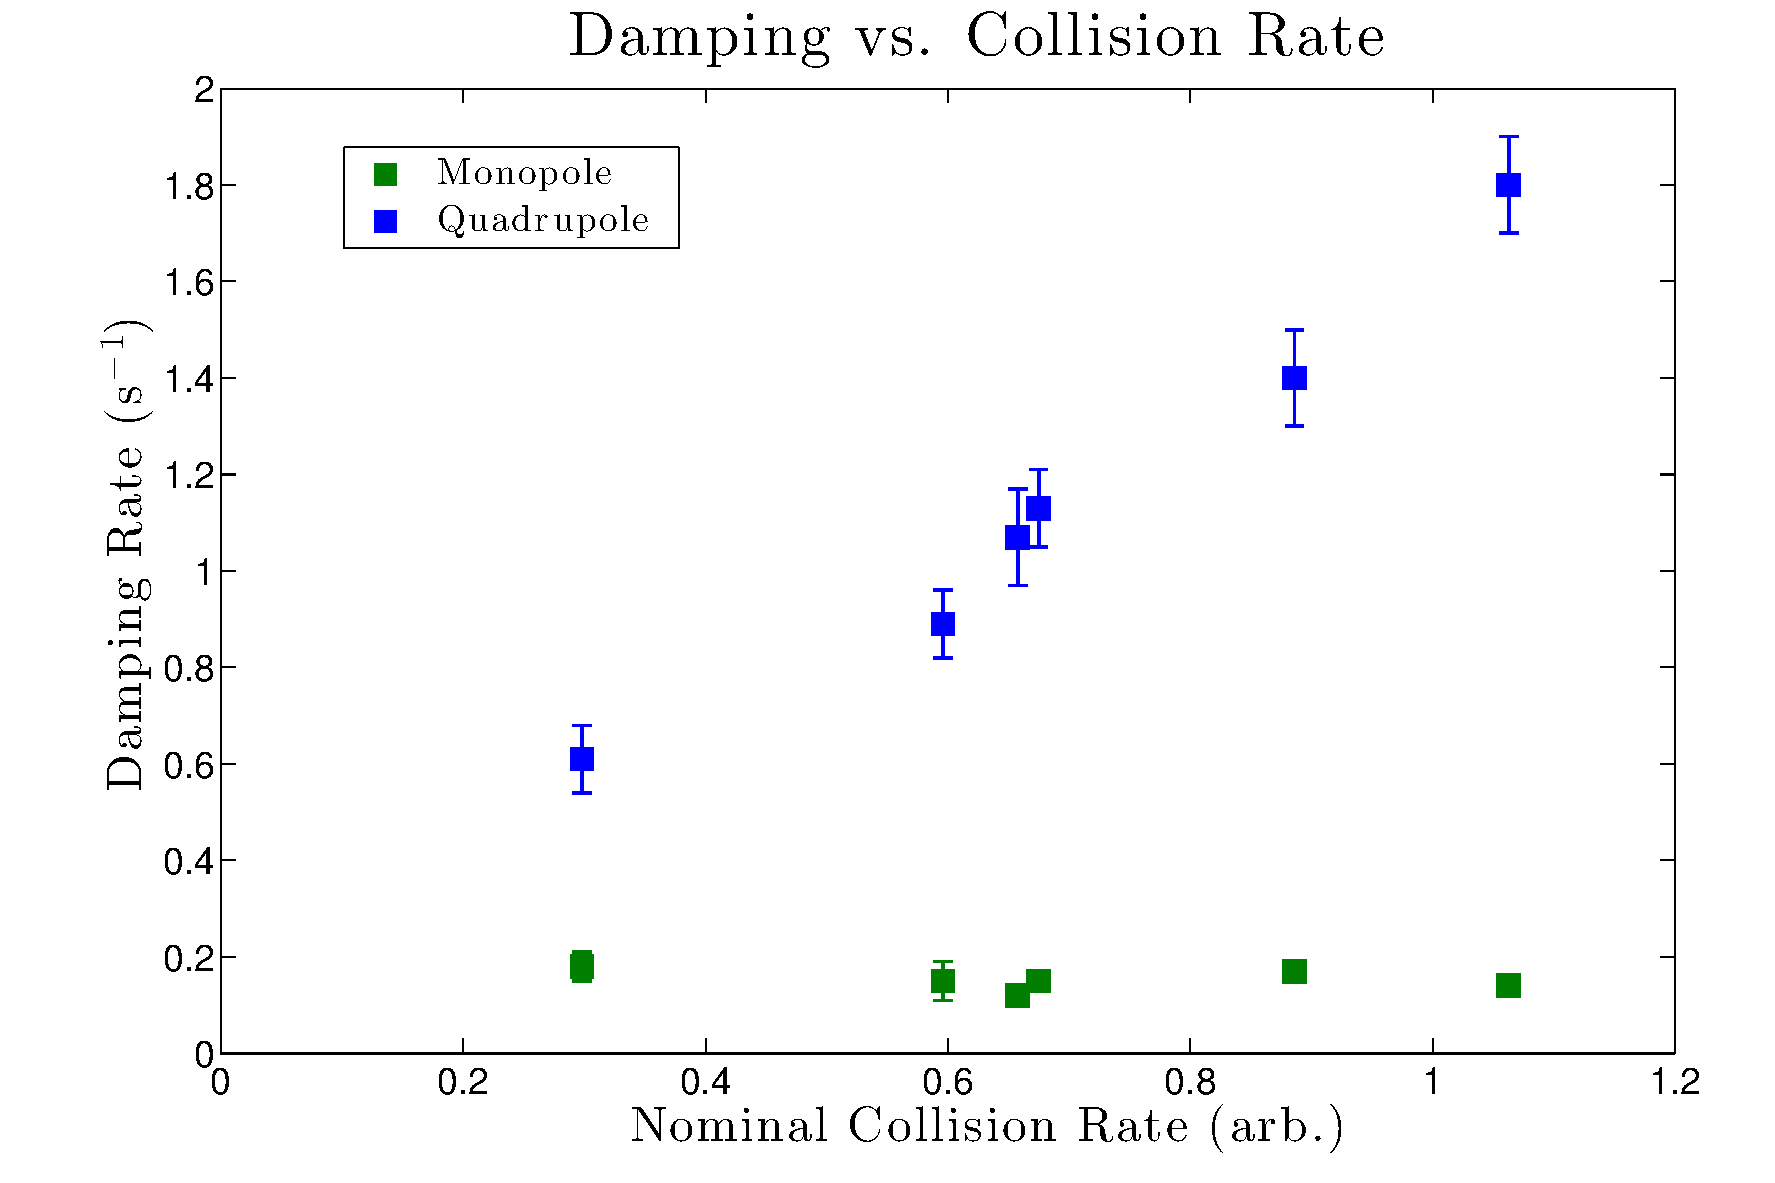
\includegraphics[width=80mm]{./figs/DampingvsCollRateSpherical_v2.pdf}
    \end{center}
    \caption[dampsphere]{
        Sample data for a driven quadrupole mode and monopole mode in a spherical trap.
        Black lines on the quadrupole data indicate a typical fitting procedure where individual periods taken in a single run are fit with an undamped sine wave to extract the amplitude.
    }
    \label{pyramid}
\end{figure}




\paragraph{A few notes on \texttt{tag}s} 
\verb+\tag{#1}+ requires the \texttt{amsmath} package. 
Place the \verb+\tag{#1}+ command before the \verb+\label{#1}+, if any. 
The numbering produced by \verb+\tag{#1}+ \textit{does not affect} 
the automatic numbering in REV\TeX; 
therefore, the number must be known ahead of time, 
and it must be manually adjusted if other equations are added. 
\verb+\tag{#1}+ works with both single-line and multiline equations. 
\verb+\tag{#1}+ should only be used in exceptional cases---%
do not use it to number many equations in your paper. 
Please note that this feature of the \texttt{amsmath} package
is \emph{not} compatible with the \texttt{hyperref} (6.77u) package.

Enclosing display math within
\verb+\begin{subequations}+ and \verb+\end{subequations}+ will produce
a set of equations that are labeled with letters, as shown in
Eqs.~(\ref{subeq:1}) and (\ref{subeq:2}) below.
You may include any number of single-line and multiline equations,
although it is probably not a good idea to follow one display math
directly after another.
\begin{subequations}
\label{eq:whole}
\begin{eqnarray}
{\cal M}=&&ig_Z^2(4E_1E_2)^{1/2}(l_i^2)^{-1}
(g_{\sigma_2}^e)^2\chi_{-\sigma_2}(p_2)\nonumber\\
&&\times
[\epsilon_i]_{\sigma_1}\chi_{\sigma_1}(p_1).\label{subeq:2}
\end{eqnarray}
\begin{equation}
\left\{
 abc123456abcdef\alpha\beta\gamma\delta1234556\alpha\beta
 \frac{1\sum^{a}_{b}}{A^2}
\right\},\label{subeq:1}
\end{equation}
\end{subequations}
Giving a \verb+\label{#1}+ command directly after the \verb+\begin{subequations}+, 
allows you to reference all the equations in the \texttt{subequations} environment. 
For example, the equations in the preceding subequations environment were
Eqs.~(\ref{eq:whole}).

\subsubsection{Wide equations}
The equation that follows is set in a wide format, i.e., it spans the full page. 
The wide format is reserved for long equations
that cannot easily be set in a single column:
\begin{widetext}
\begin{equation}
{\cal R}^{(\text{d})}=
 g_{\sigma_2}^e
 \left(
   \frac{[\Gamma^Z(3,21)]_{\sigma_1}}{Q_{12}^2-M_W^2}
  +\frac{[\Gamma^Z(13,2)]_{\sigma_1}}{Q_{13}^2-M_W^2}
 \right)
 + x_WQ_e
 \left(
   \frac{[\Gamma^\gamma(3,21)]_{\sigma_1}}{Q_{12}^2-M_W^2}
  +\frac{[\Gamma^\gamma(13,2)]_{\sigma_1}}{Q_{13}^2-M_W^2}
 \right)\;. 
 \label{eq:wideeq}
\end{equation}
\end{widetext}
This is typed to show how the output appears in wide format.
(Incidentally, since there is no blank line between the \texttt{equation} environment above 
and the start of this paragraph, this paragraph is not indented.)

\section{Cross-referencing}
REV\TeX{} will automatically number such things as
sections, footnotes, equations, figure captions, and table captions. 
In order to reference them in text, use the
\verb+\label{#1}+ and \verb+\ref{#1}+ commands. 
To reference a particular page, use the \verb+\pageref{#1}+ command.

The \verb+\label{#1}+ should appear 
within the section heading, 
within the footnote text, 
within the equation, or 
within the table or figure caption. 
The \verb+\ref{#1}+ command
is used in text at the point where the reference is to be displayed.  
Some examples: Section~\ref{sec:level1} on page~\pageref{sec:level1},
Table~\ref{tab:table1},%
\begin{table}[b]%The best place to locate the table environment is directly after its first reference in text
\caption{\label{tab:table1}%
A table that fits into a single column of a two-column layout. 
Note that REV\TeX~4 adjusts the intercolumn spacing so that the table fills the
entire width of the column. Table captions are numbered
automatically. 
This table illustrates left-, center-, decimal- and right-aligned columns,
along with the use of the \texttt{ruledtabular} environment which sets the 
Scotch (double) rules above and below the alignment, per APS style.
}
\begin{ruledtabular}
\begin{tabular}{lcdr}
\textrm{Left\footnote{Note a.}}&
\textrm{Centered\footnote{Note b.}}&
\multicolumn{1}{c}{\textrm{Decimal}}&
\textrm{Right}\\
\colrule
1 & 2 & 3.001 & 4\\
10 & 20 & 30 & 40\\
100 & 200 & 300.0 & 400\\
\end{tabular}
\end{ruledtabular}
\end{table}
and Fig.~\ref{fig:epsart}.%
\begin{figure}[b]
\includegraphics{fig_1}% Here is how to import EPS art
\caption{\label{fig:epsart} A figure caption. The figure captions are
automatically numbered.}
\end{figure}

\section{Floats: Figures, Tables, Videos, etc.}
Figures and tables are usually allowed to ``float'', which means that their
placement is determined by \LaTeX, while the document is being typeset. 

Use the \texttt{figure} environment for a figure, the \texttt{table} environment for a table.
In each case, use the \verb+\caption+ command within to give the text of the
figure or table caption along with the \verb+\label+ command to provide
a key for referring to this figure or table.
The typical content of a figure is an image of some kind; 
that of a table is an alignment.%
\begin{figure*}
\includegraphics{fig_2}% Here is how to import EPS art
\caption{\label{fig:wide}Use the figure* environment to get a wide
figure that spans the page in \texttt{twocolumn} formatting.}
\end{figure*}
\begin{table*}
\caption{\label{tab:table3}This is a wide table that spans the full page
width in a two-column layout. It is formatted using the
\texttt{table*} environment. It also demonstates the use of
\textbackslash\texttt{multicolumn} in rows with entries that span
more than one column.}
\begin{ruledtabular}
\begin{tabular}{ccccc}
 &\multicolumn{2}{c}{$D_{4h}^1$}&\multicolumn{2}{c}{$D_{4h}^5$}\\
 Ion&1st alternative&2nd alternative&lst alternative
&2nd alternative\\ \hline
 K&$(2e)+(2f)$&$(4i)$ &$(2c)+(2d)$&$(4f)$ \\
 Mn&$(2g)$\footnote{The $z$ parameter of these positions is $z\sim\frac{1}{4}$.}
 &$(a)+(b)+(c)+(d)$&$(4e)$&$(2a)+(2b)$\\
 Cl&$(a)+(b)+(c)+(d)$&$(2g)$\footnotemark[1]
 &$(4e)^{\text{a}}$\\
 He&$(8r)^{\text{a}}$&$(4j)^{\text{a}}$&$(4g)^{\text{a}}$\\
 Ag& &$(4k)^{\text{a}}$& &$(4h)^{\text{a}}$\\
\end{tabular}
\end{ruledtabular}
\end{table*}

Insert an image using either the \texttt{graphics} or
\texttt{graphix} packages, which define the \verb+\includegraphics{#1}+ command.
(The two packages differ in respect of the optional arguments 
used to specify the orientation, scaling, and translation of the image.) 
To create an alignment, use the \texttt{tabular} environment. 

The best place to locate the \texttt{figure} or \texttt{table} environment
is immediately following its first reference in text; this sample document
illustrates this practice for Fig.~\ref{fig:epsart}, which
shows a figure that is small enough to fit in a single column. 

In exceptional cases, you will need to move the float earlier in the document, as was done
with Table~\ref{tab:table3}: \LaTeX's float placement algorithms need to know
about a full-page-width float earlier. 

Fig.~\ref{fig:wide}
has content that is too wide for a single column,
so the \texttt{figure*} environment has been used.%
\begin{table}[b]
\caption{\label{tab:table4}%
Numbers in columns Three--Five are aligned with the ``d'' column specifier 
(requires the \texttt{dcolumn} package). 
Non-numeric entries (those entries without a ``.'') in a ``d'' column are aligned on the decimal point. 
Use the ``D'' specifier for more complex layouts. }
\begin{ruledtabular}
\begin{tabular}{ccddd}
One&Two&
\multicolumn{1}{c}{\textrm{Three}}&
\multicolumn{1}{c}{\textrm{Four}}&
\multicolumn{1}{c}{\textrm{Five}}\\
%\mbox{Three}&\mbox{Four}&\mbox{Five}\\
\hline
one&two&\mbox{three}&\mbox{four}&\mbox{five}\\
He&2& 2.77234 & 45672. & 0.69 \\
C\footnote{Some tables require footnotes.}
  &C\footnote{Some tables need more than one footnote.}
  & 12537.64 & 37.66345 & 86.37 \\
\end{tabular}
\end{ruledtabular}
\end{table}

The content of a table is typically a \texttt{tabular} environment, 
giving rows of type in aligned columns. 
Column entries separated by \verb+&+'s, and 
each row ends with \textbackslash\textbackslash. 
The required argument for the \texttt{tabular} environment
specifies how data are aligned in the columns. 
For instance, entries may be centered, left-justified, right-justified, aligned on a decimal
point. 
Extra column-spacing may be be specified as well, 
although REV\TeX~4 sets this spacing so that the columns fill the width of the
table. Horizontal rules are typeset using the \verb+\hline+
command. The doubled (or Scotch) rules that appear at the top and
bottom of a table can be achieved enclosing the \texttt{tabular}
environment within a \texttt{ruledtabular} environment. Rows whose
columns span multiple columns can be typeset using the
\verb+\multicolumn{#1}{#2}{#3}+ command (for example, see the first
row of Table~\ref{tab:table3}).%

Tables~\ref{tab:table1}, \ref{tab:table3}, \ref{tab:table4}, and \ref{tab:table2}%
\begin{table}[b]
\caption{\label{tab:table2}
A table with numerous columns that still fits into a single column. 
Here, several entries share the same footnote. 
Inspect the \LaTeX\ input for this table to see exactly how it is done.}
\begin{ruledtabular}
\begin{tabular}{cccccccc}
 &$r_c$ (\AA)&$r_0$ (\AA)&$\kappa r_0$&
 &$r_c$ (\AA) &$r_0$ (\AA)&$\kappa r_0$\\
\hline
Cu& 0.800 & 14.10 & 2.550 &Sn\footnotemark[1]
& 0.680 & 1.870 & 3.700 \\
Ag& 0.990 & 15.90 & 2.710 &Pb\footnotemark[2]
& 0.450 & 1.930 & 3.760 \\
Au& 1.150 & 15.90 & 2.710 &Ca\footnotemark[3]
& 0.750 & 2.170 & 3.560 \\
Mg& 0.490 & 17.60 & 3.200 &Sr\footnotemark[4]
& 0.900 & 2.370 & 3.720 \\
Zn& 0.300 & 15.20 & 2.970 &Li\footnotemark[2]
& 0.380 & 1.730 & 2.830 \\
Cd& 0.530 & 17.10 & 3.160 &Na\footnotemark[5]
& 0.760 & 2.110 & 3.120 \\
Hg& 0.550 & 17.80 & 3.220 &K\footnotemark[5]
&  1.120 & 2.620 & 3.480 \\
Al& 0.230 & 15.80 & 3.240 &Rb\footnotemark[3]
& 1.330 & 2.800 & 3.590 \\
Ga& 0.310 & 16.70 & 3.330 &Cs\footnotemark[4]
& 1.420 & 3.030 & 3.740 \\
In& 0.460 & 18.40 & 3.500 &Ba\footnotemark[5]
& 0.960 & 2.460 & 3.780 \\
Tl& 0.480 & 18.90 & 3.550 & & & & \\
\end{tabular}
\end{ruledtabular}
\footnotetext[1]{Here's the first, from Ref.~\onlinecite{feyn54}.}
\footnotetext[2]{Here's the second.}
\footnotetext[3]{Here's the third.}
\footnotetext[4]{Here's the fourth.}
\footnotetext[5]{And etc.}
\end{table}
show various effects.
A table that fits in a single column employs the \texttt{table}
environment. 
Table~\ref{tab:table3} is a wide table, set with the \texttt{table*} environment. 
Long tables may need to break across pages. 
The most straightforward way to accomplish this is to specify
the \verb+[H]+ float placement on the \texttt{table} or
\texttt{table*} environment. 
However, the \LaTeXe\ package \texttt{longtable} allows headers and footers to be specified for each page of the table. 
A simple example of the use of \texttt{longtable} can be found
in the file \texttt{summary.tex} that is included with the REV\TeX~4
distribution.

There are two methods for setting footnotes within a table (these
footnotes will be displayed directly below the table rather than at
the bottom of the page or in the bibliography). The easiest
and preferred method is just to use the \verb+\footnote{#1}+
command. This will automatically enumerate the footnotes with
lowercase roman letters. However, it is sometimes necessary to have
multiple entries in the table share the same footnote. In this case,
there is no choice but to manually create the footnotes using
\verb+\footnotemark[#1]+ and \verb+\footnotetext[#1]{#2}+.
\texttt{\#1} is a numeric value. Each time the same value for
\texttt{\#1} is used, the same mark is produced in the table. The
\verb+\footnotetext[#1]{#2}+ commands are placed after the \texttt{tabular}
environment. Examine the \LaTeX\ source and output for
Tables~\ref{tab:table1} and \ref{tab:table2}
for examples.

Video~\ref{vid:PRSTPER.4.010101} 
illustrates several features new with REV\TeX4.1,
starting with the \texttt{video} environment, which is in the same category with
\texttt{figure} and \texttt{table}.%
\begin{video}
\href{http://prst-per.aps.org/multimedia/PRSTPER/v4/i1/e010101/e010101_vid1a.mpg}{\includegraphics{vid_1a}}%
 \quad
\href{http://prst-per.aps.org/multimedia/PRSTPER/v4/i1/e010101/e010101_vid1b.mpg}{\includegraphics{vid_1b}}
 \setfloatlink{http://link.aps.org/multimedia/PRSTPER/v4/i1/e010101}%
 \caption{\label{vid:PRSTPER.4.010101}%
  Students explain their initial idea about Newton's third law to a teaching assistant. 
  Clip (a): same force.
  Clip (b): move backwards.
 }%
\end{video}
The \verb+\setfloatlink+ command causes the title of the video to be a hyperlink to the
indicated URL; it may be used with any environment that takes the \verb+\caption+
command.
The \verb+\href+ command has the same significance as it does in the context of
the \texttt{hyperref} package: the second argument is a piece of text to be 
typeset in your document; the first is its hyperlink, a URL.

\textit{Physical Review} style requires that the initial citation of
figures or tables be in numerical order in text, so don't cite
Fig.~\ref{fig:wide} until Fig.~\ref{fig:epsart} has been cited.

\begin{acknowledgments}
We wish to acknowledge the support of the author community in using
REV\TeX{}, offering suggestions and encouragement, testing new versions,
\dots.
\end{acknowledgments}

\appendix

\section{Appendixes}

To start the appendixes, use the \verb+\appendix+ command.
This signals that all following section commands refer to appendixes
instead of regular sections. Therefore, the \verb+\appendix+ command
should be used only once---to setup the section commands to act as
appendixes. Thereafter normal section commands are used. The heading
for a section can be left empty. For example,
\begin{verbatim}
\appendix
\section{}
\end{verbatim}
will produce an appendix heading that says ``APPENDIX A'' and
\begin{verbatim}
\appendix
\section{Background}
\end{verbatim}
will produce an appendix heading that says ``APPENDIX A: BACKGROUND''
(note that the colon is set automatically).

If there is only one appendix, then the letter ``A'' should not
appear. This is suppressed by using the star version of the appendix
command (\verb+\appendix*+ in the place of \verb+\appendix+).

\section{A little more on appendixes}

Observe that this appendix was started by using
\begin{verbatim}
\section{A little more on appendixes}
\end{verbatim}

Note the equation number in an appendix:
\begin{equation}
E=mc^2.
\end{equation}

\subsection{\label{app:subsec}A subsection in an appendix}

You can use a subsection or subsubsection in an appendix. Note the
numbering: we are now in Appendix~\ref{app:subsec}.

Note the equation numbers in this appendix, produced with the
subequations environment:
\begin{subequations}
\begin{eqnarray}
E&=&mc, \label{appa}
\\
E&=&mc^2, \label{appb}
\\
E&\agt& mc^3. \label{appc}
\end{eqnarray}
\end{subequations}
They turn out to be Eqs.~(\ref{appa}), (\ref{appb}), and (\ref{appc}).

% The \nocite command causes all entries in a bibliography to be printed out
% whether or not they are actually referenced in the text. This is appropriate
% for the sample file to show the different styles of references, but authors
% most likely will not want to use it.
\nocite{*}

\bibliography{apssamp}% Produces the bibliography via BibTeX.

\end{document}
%
% ****** End of file apssamp.tex ******
